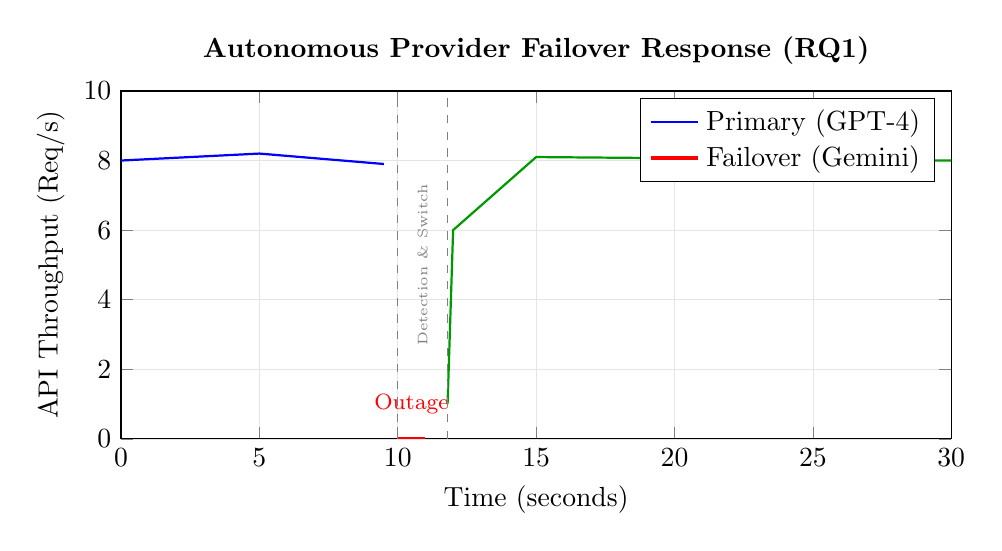
\begin{tikzpicture}
\begin{axis}[
    width=\columnwidth,
    height=6cm,
    xlabel={Time (seconds)},
    ylabel={API Throughput (Req/s)},
    xmin=0, xmax=30,
    ymin=0, ymax=10,
    grid=both,
    grid style={line width=.1pt, draw=gray!10},
    major grid style={line width=.2pt, draw=gray!20},
    title={\textbf{Autonomous Provider Failover Response (RQ1)}}
]
    % Normal operation
    \addplot[blue, thick] coordinates {(0, 8) (5, 8.2) (9.5, 7.9)};
    
    % Outage
    \addplot[red, ultra thick] coordinates {(10, 0) (11, 0)};
    \node[red, font=\footnotesize] at (axis cs:10.5, 1) {Outage};
    
    % Failover spike and recovery
    \addplot[green!60!black, thick] coordinates {(11.8, 1) (12, 6) (15, 8.1) (30, 8)};
    
    \draw[dashed, gray] (axis cs:10, 0) -- (axis cs:10, 10);
    \draw[dashed, gray] (axis cs:11.8, 0) -- (axis cs:11.8, 10);
    \node[gray, font=\tiny, rotate=90] at (axis cs:10.9, 5) {Detection \& Switch};

    \legend{Primary (GPT-4), Failover (Gemini)}
\end{axis}
\end{tikzpicture}
